\headline{{\textbf{\Large\sffamily Bonsai Roots:}}\\
{\textbf{\large\sffamily Meet the Members of TWBC}}}
\label{2025-07-roots}
\noindent
In every edition of \emph{Bonsai Roots,} we step away from wiring and watering for a moment to celebrate the members who make our club so special.
Everyone's story adds a new leaf to the rich tapestry of TWBC.
This month, we're delighted to introduce \textbf{Grant Kinnaird}, a bonsai enthusiast with thirty years of experience and a love for hardy species!

\begin{itemize}
    \item \textbf{What's your name and where in the country do you live?}

    \emph{I'm Grant, living in South London---a great area for bonsai, with plenty of nurseries and like\--minded enthusiasts nearby.}

    \item \textbf{What are your favourite species of tree and why?}

    \emph{I particularly enjoy working with Larch and Hawthorn. They're hardy trees that respond well to training, and they've always given me rewarding results over the years.}

    \item \textbf{What aspect of bonsai do you enjoy?}

    \emph{Developing Yamadori is my favourite part---there's something special about shaping wild\--collected trees and bringing out their natural character.}

    \item \textbf{What aspects of bonsai do you find most challenging?}

    \emph{Getting fertiliser right can be tricky. Even after decades, I'm still fine\--tuning my approach to feeding different species.}

    \item \textbf{Who or what inspires you throughout your bonsai journey?}

    \emph{Andrew from the Bonsai Shed has been a big inspiration --- his practical advice and deep knowledge have helped me improve my techniques.}

    \item \textbf{How long have you been interested in keeping bonsai?}

    \emph{I've been practising bonsai for about thirty years now, though I still feel like there's always more to learn.}

    \item \textbf{What stimulated your interest in bonsai?}

    \emph{The challenge of shaping trees and seeing the results over time is what first drew me in---and it's what keeps me hooked.}

    \item \textbf{If you could give someone new to bonsai any tips, what would it be?}

    \emph{Read books by experts like Dan Barton, Colin Lewis, Peter Adams, and Harry Harrington. They offer invaluable advice that's helped me avoid many early mistakes.}

    \item \textbf{Why do you enjoy being part of TWBC, and do you have any ideas or suggestions for the club's future?}

    \emph{I've only been a member for a few months, but I've already found TWBC to be a welcoming club with very knowledgeable members. It's a great place to learn and share ideas.}

    \item \textbf{One word to describe what bonsai means to you?}

    \emph{Challenging---but in the best possible way.}

    \item \textbf{What are your future goals regarding your own trees and learning more about the hobby?}

    \emph{I'd like to keep refining my trees and perhaps focus more on developing Yamadori material in the coming years.}

    \item \textbf{How would you like to see your bonsai journey progress in the future?}

    \emph{I hope to keep learning, experimenting, and most of all---enjoying the process.}
\end{itemize}

Grant's decades of experience and practical approach make him a fantastic addition to TWBC.
We look forward to seeing more of his trees in the future!
Who'll we meet next in \emph{Bonsai Roots}? Stay tuned!

\begin{center}
    $\cdots$
\end{center}

\noindent
\emph{If you're a newer member and would like to feature in a future edition of Bonsai Roots, simply fill out the form at \href{https://forms.gle/quVXa4L8rhpnT5kr6}{this link}! We'd love to hear your story.}
\closearticle

\end{multicols}

\begin{center}
    \begin{minipage}[b]{.18\textwidth}
        \includegraphics[angle=0,origin=c,width=1.0\textwidth]{2025_07/res/event/roots_01}
    \end{minipage}\quad
    \begin{minipage}[b]{.18\textwidth}
        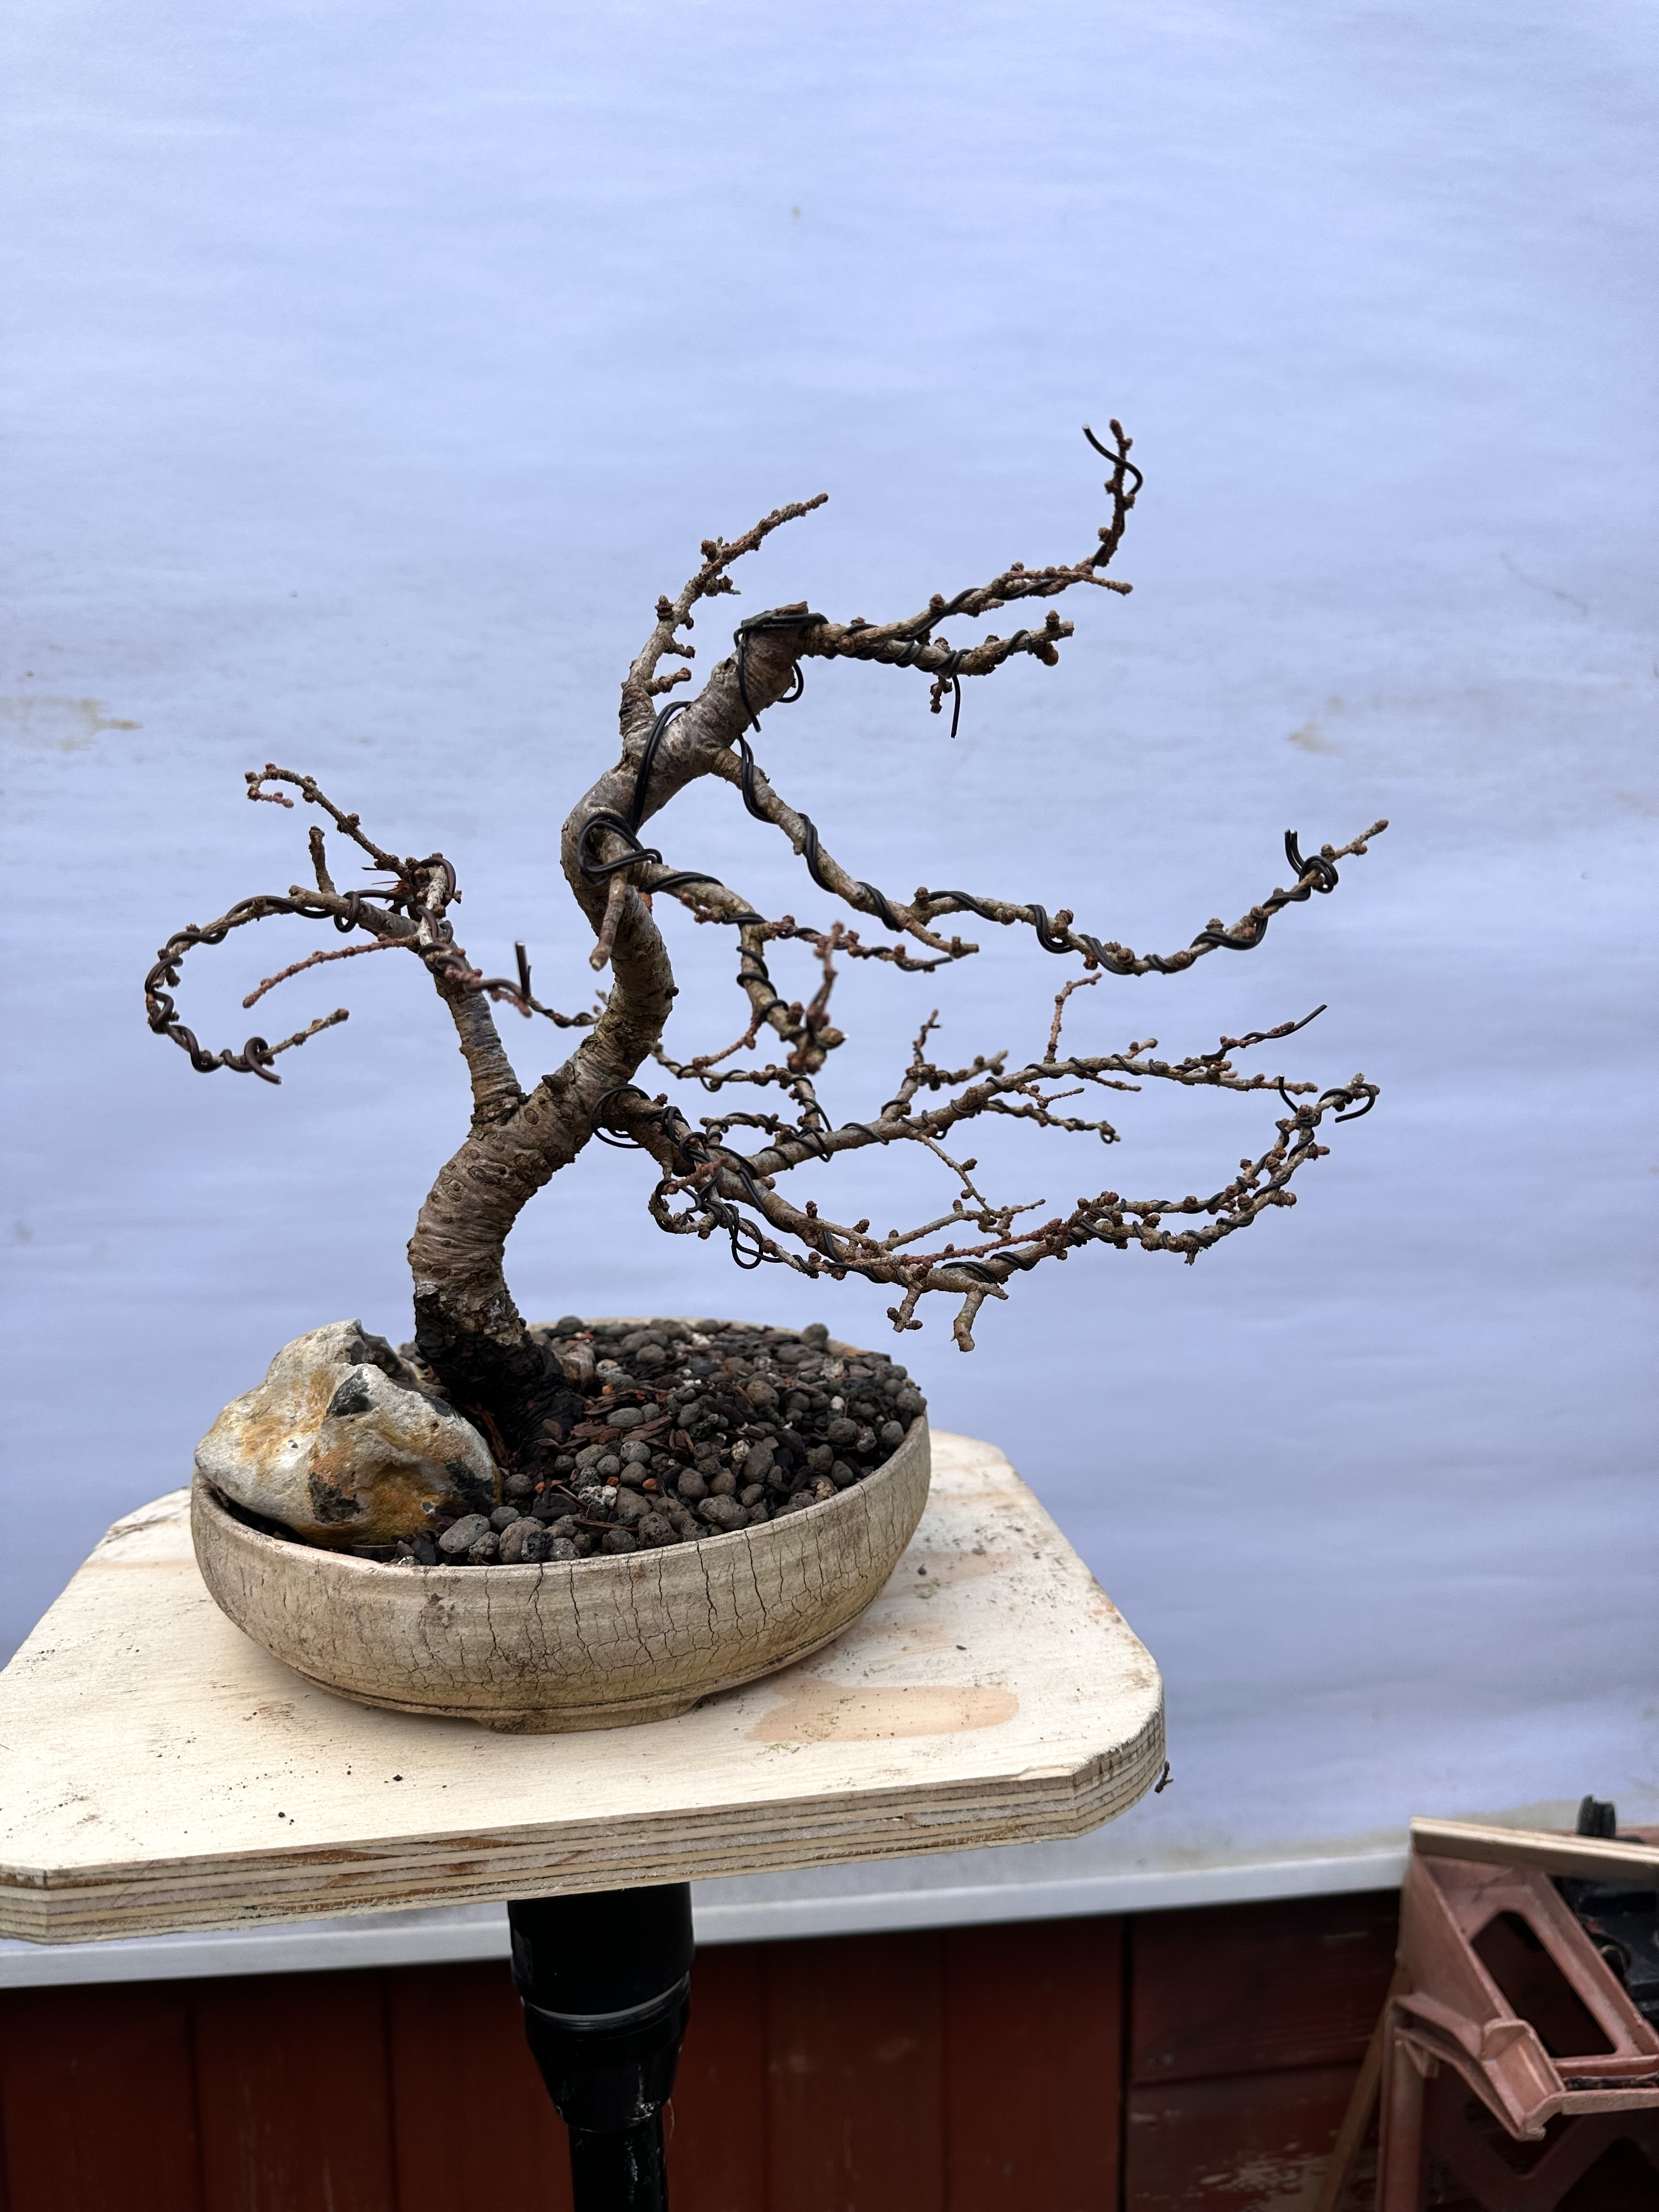
\includegraphics[angle=0,origin=c,width=1.0\textwidth]{2025_07/res/event/roots_02}
    \end{minipage}\quad
    \begin{minipage}[b]{.18\textwidth}
        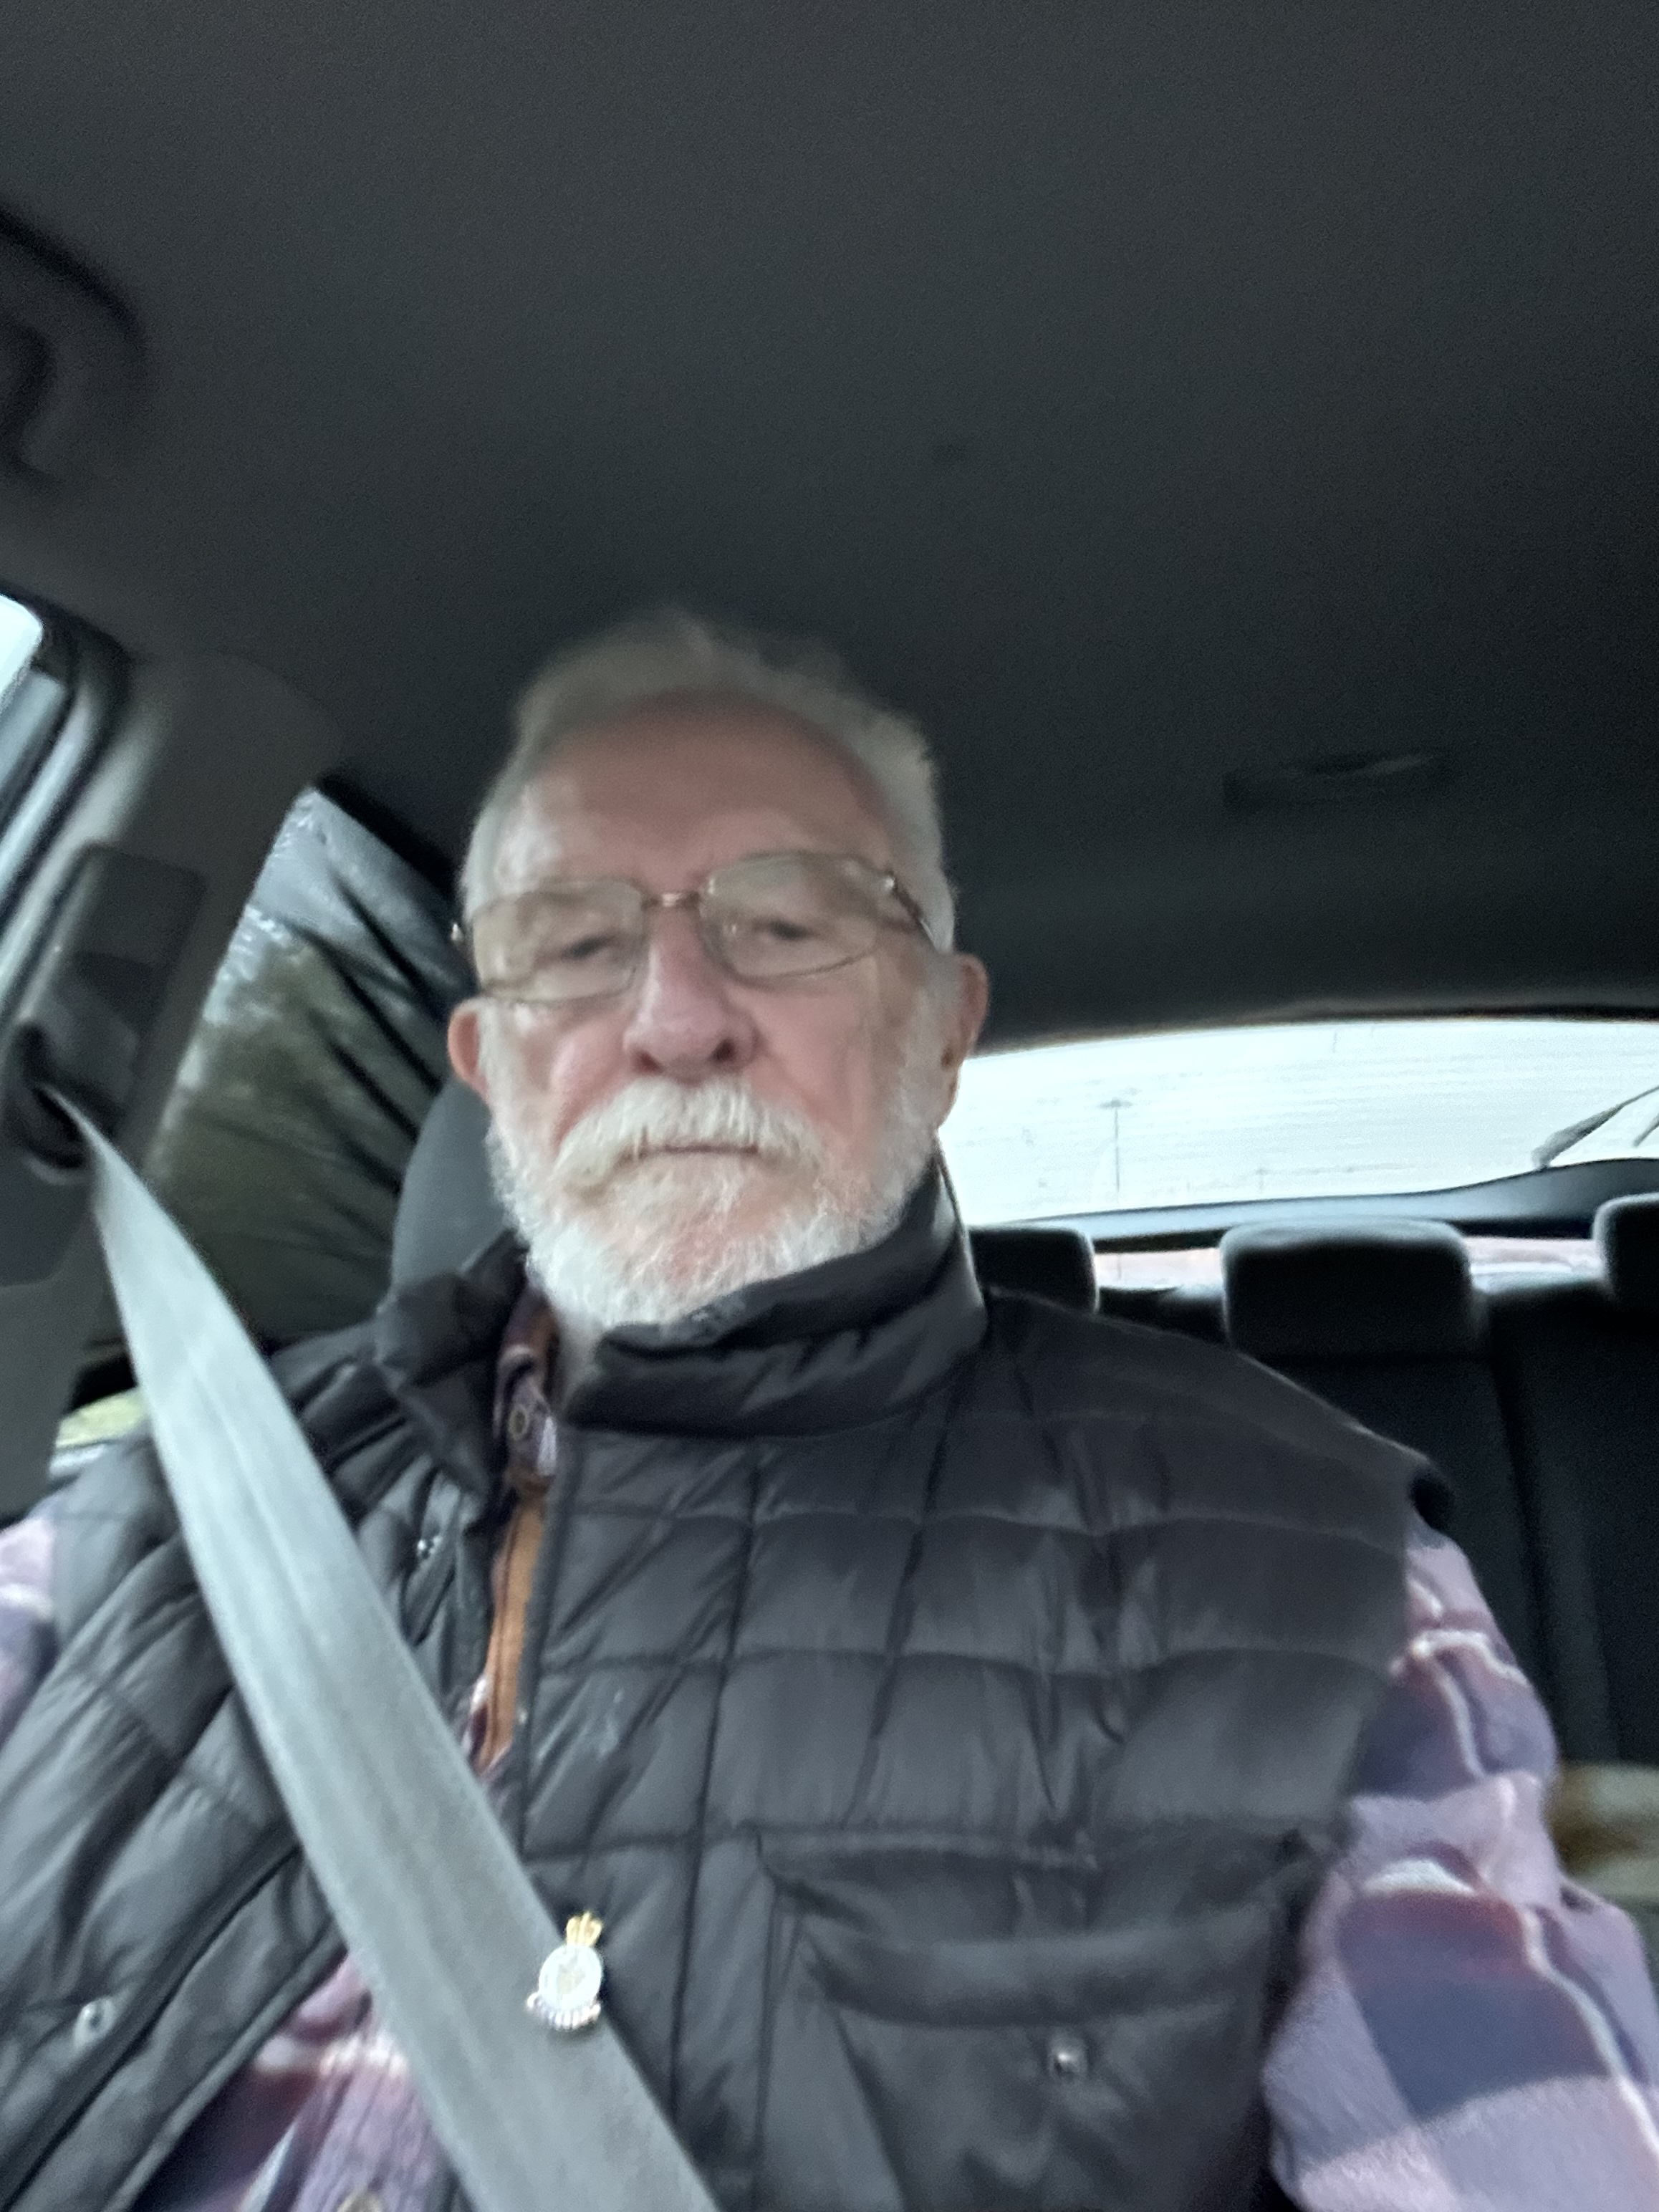
\includegraphics[angle=0,origin=c,width=1.0\textwidth]{2025_07/res/event/roots_03}
    \end{minipage}\quad
    \begin{minipage}[b]{.18\textwidth}
        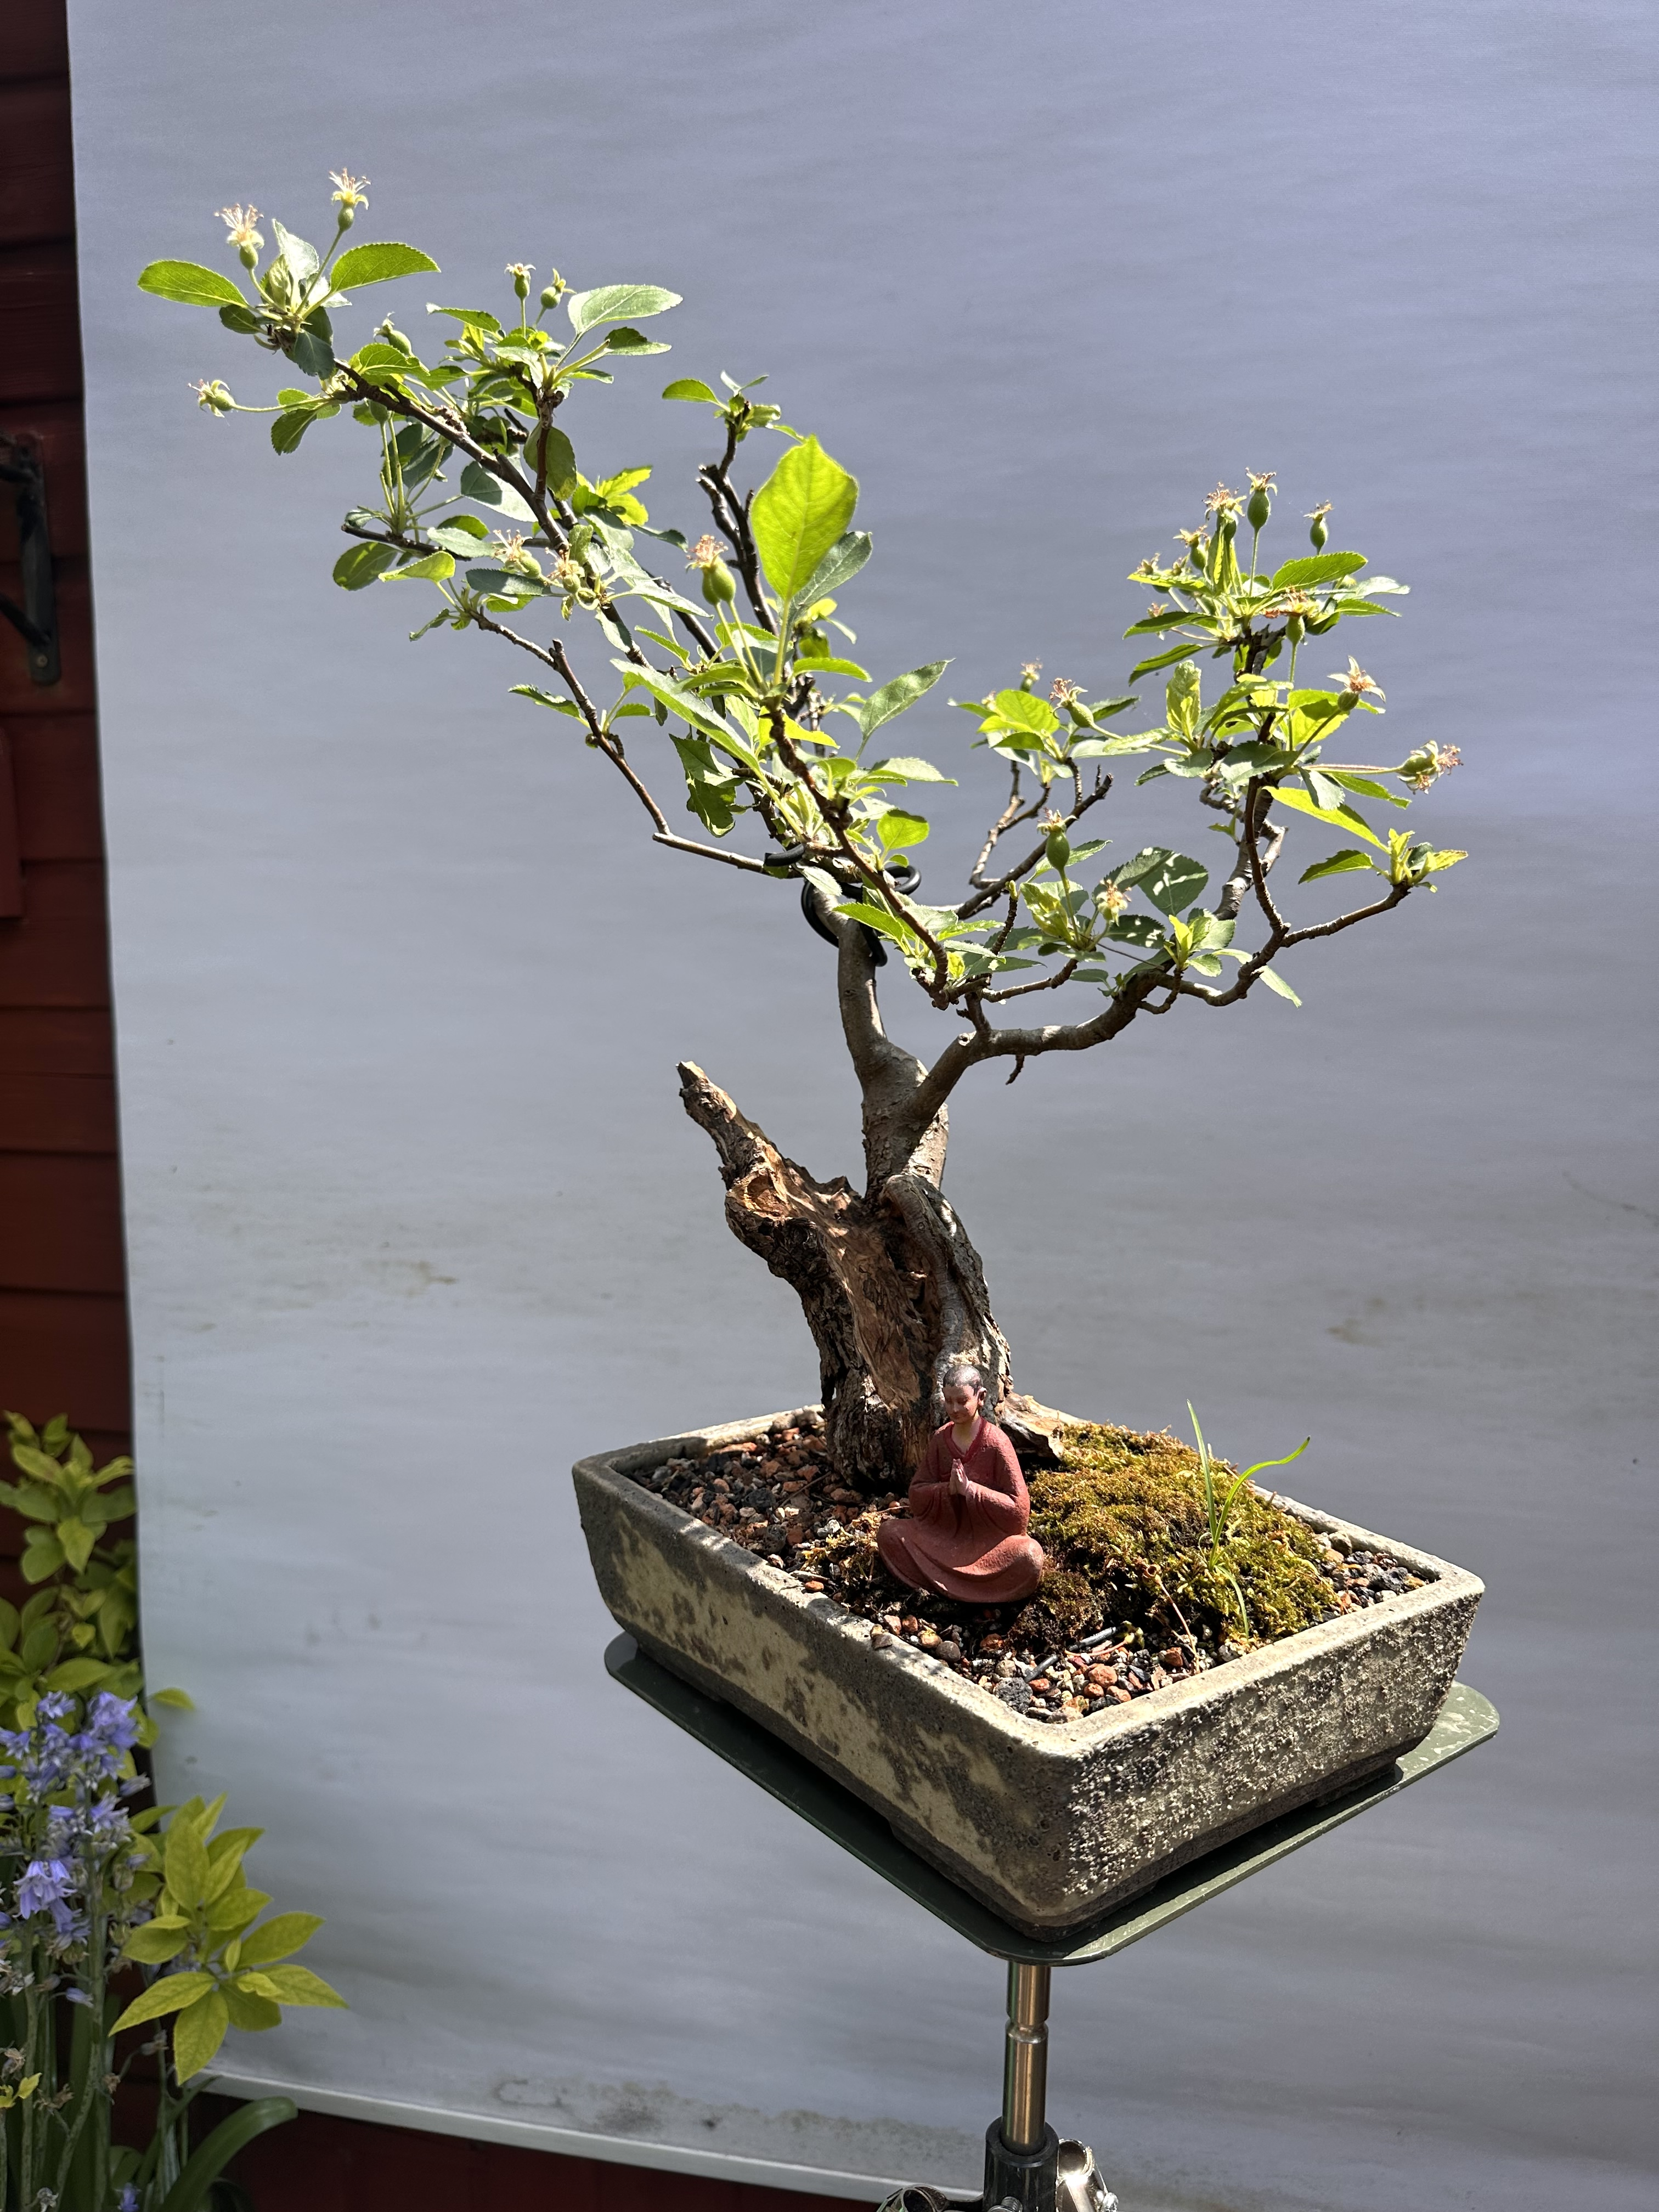
\includegraphics[angle=0,origin=c,width=1.0\textwidth]{2025_07/res/event/roots_04}
    \end{minipage}\quad
    \begin{minipage}[b]{.18\textwidth}
        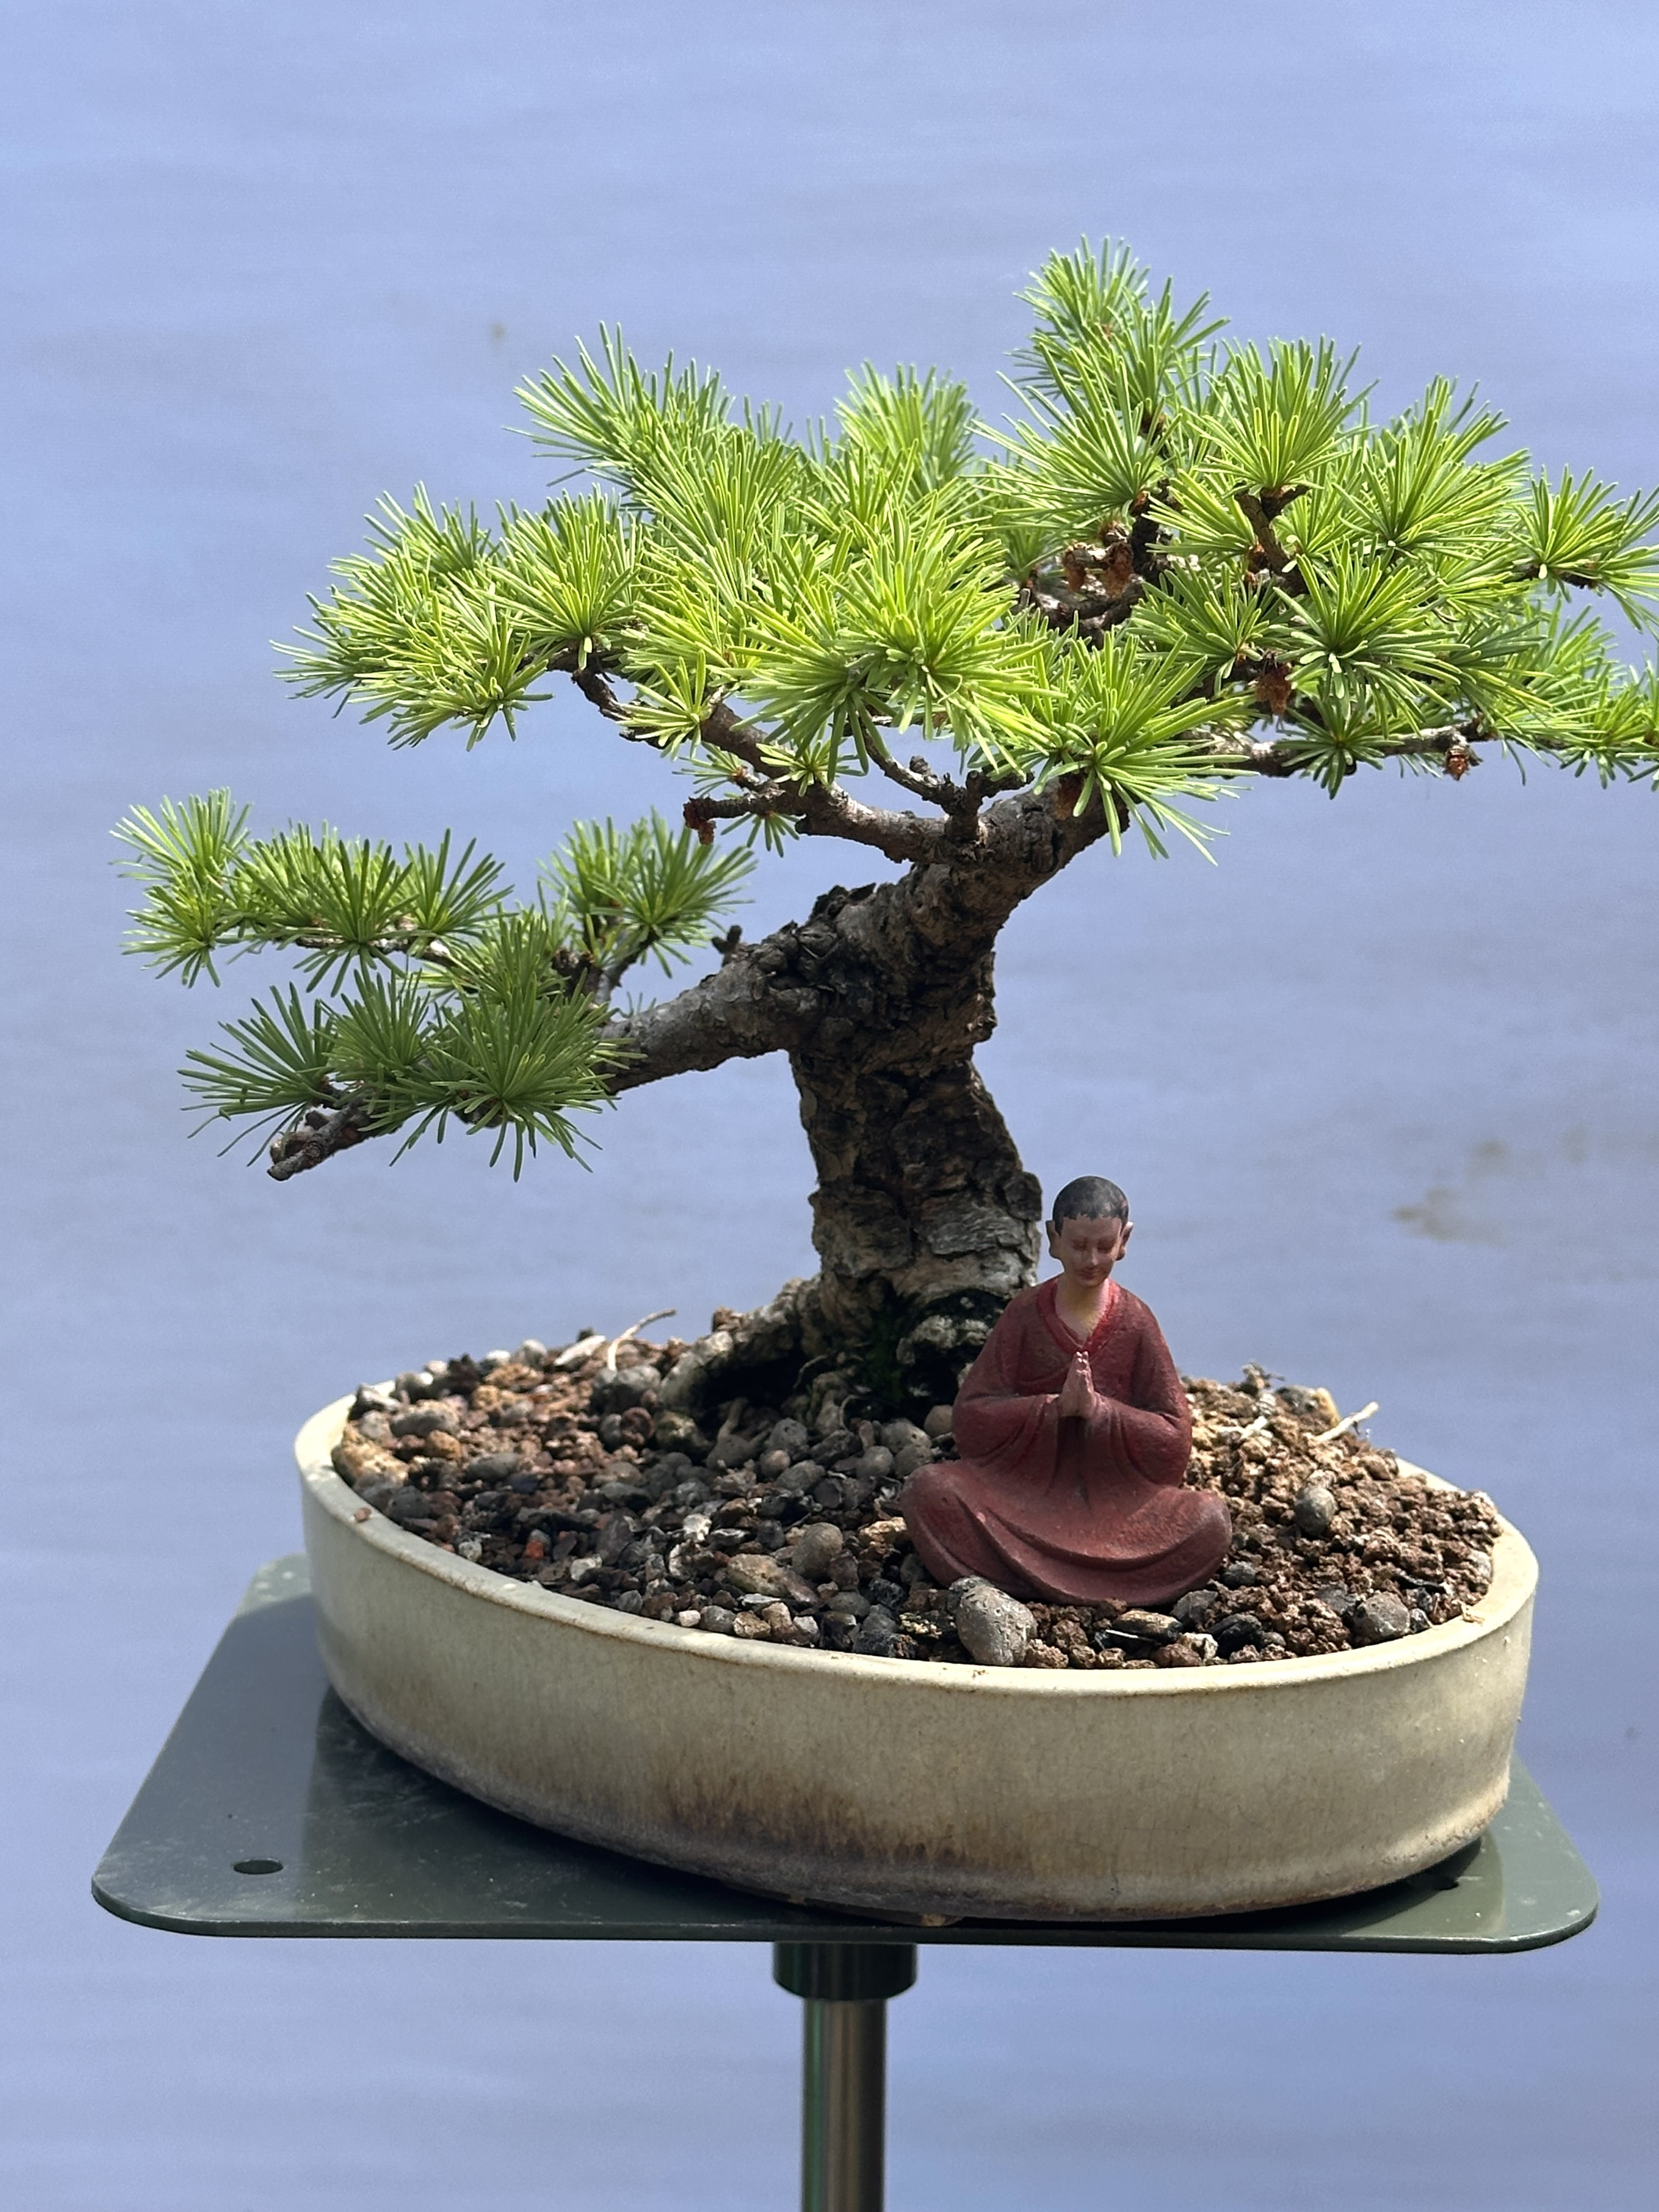
\includegraphics[angle=0,origin=c,width=1.0\textwidth]{2025_07/res/event/roots_05}
    \end{minipage}
    \medskip
    \emph{Grant Kinnaird surrounded by some of his most charming Shohin trees.}
\end{center}

\begin{multicols}{2}

\clearpage
